\section{Design sekvens-diagram}
\todo[inline]{Chris: tegn diagram og forklar}
\begin{figure}[!ht]
\centering
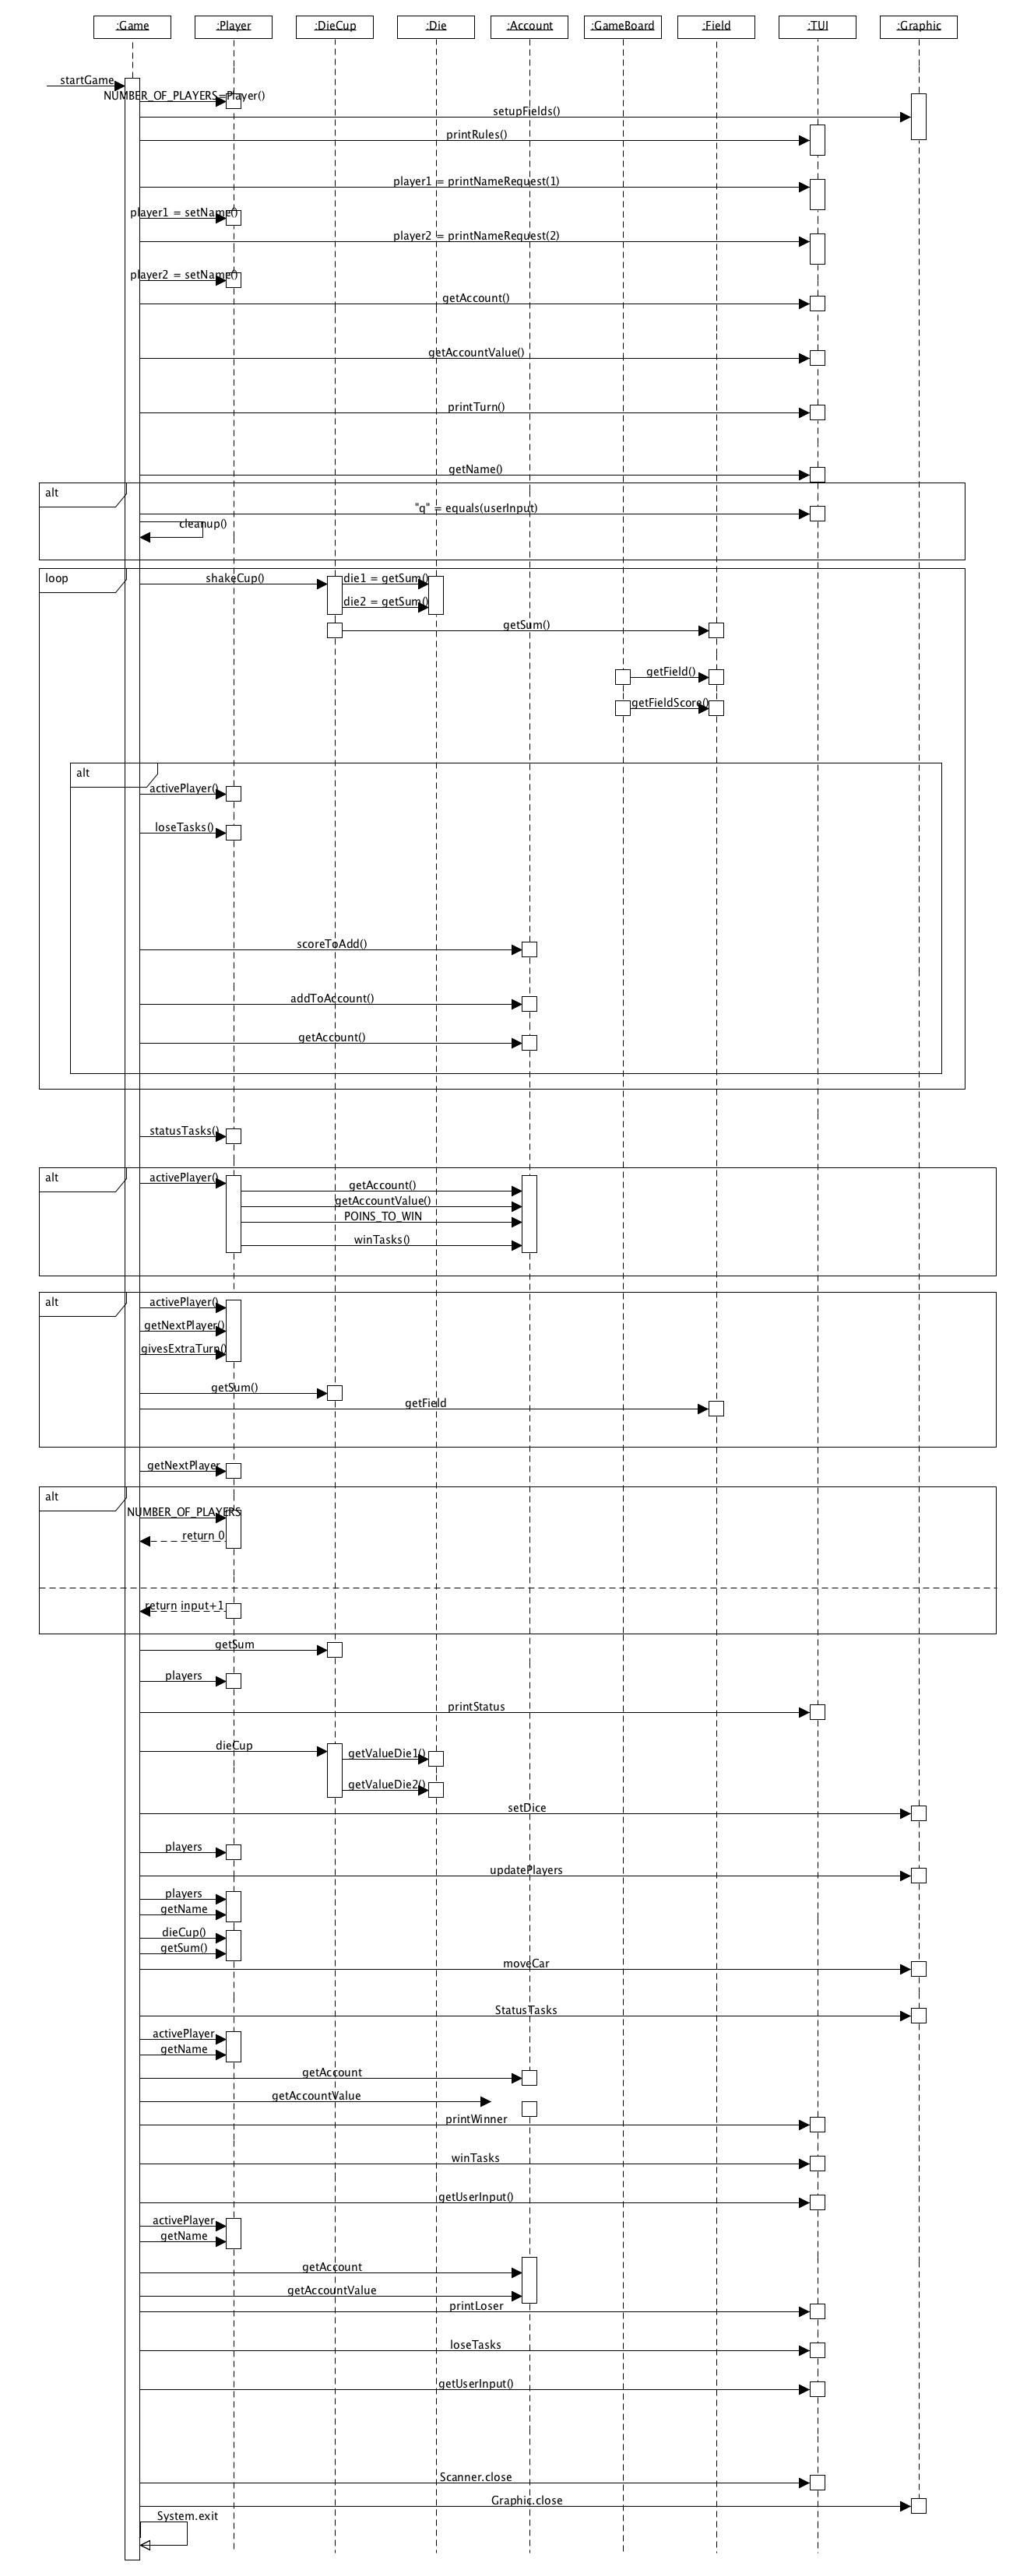
\includegraphics[scale=0.14]{DesignSequenceDiagram.jpg}
\caption[<Text for the list of figures>]{Design Sekvens Diagram}
\label{fig:figure2}
\end{figure}
\newpage
Vi har, som ved første spil,  lavet et design sekvens-diagram, som dokumenterer, hvordan koden bliver udført sekventielt, når man spiller det nye feltspil. Hvis man sammenligner vores sekvensdiagram med vores kode afsnit, vil man se at \textit{Game} controlleren har det primære ansvar for at fordele opgaverne rundt til de ande dele af programmet. Her kan vi bare se det ud fra et tidsmæssigt perspektiv istedet. Hvordan de forskellige metodekald virker, kan man nærstudere i vores afsnit om selve koden.
\\

Desværre er diagrammet fyldt med forkert syntaks og variabler, der er brugt som metodekald. Da dette er noget af det sidste vi har lavet i vores dokumentation, har tidsgrænsen bevirket, vi ikke har kunnet afhjælpe disse fejl inden for den ønskede tidsramme.
\\
Vi vil dog anbefale, at man får dette rettet hurtigst muligt, hvis der er planer om eventuelle opdateringer til spillet, eller genbrug af dele af systemet.